\section{Topological data analysis}
Topological Data Analysis (TDA) is a fast growing field of mathematics, providing a set of tools from topology in order to infer underlying features from data \cite{chazal2021introduction}. In this section, we will go over the concepts of TDA, such as simplicial complexes or persistence diagrams. Then, we will introduce a couple of algorithms which uses concepts from TDA. This section is based on \cites{Edelsbrunner2010}{chazal2021introduction}, if not stated otherwise.

\subsection{Simplicial complex}
\label{sec:simplicial-complex}
In computer science, a graph is a datatype for describing possibly non-linear and complex relationships between data points. Graphs consist of vertices that are connected by edges. Edges can also have metadata such as weight and direction. An example of a commonly used graph is the k-nearest neighbour graph, where vertices are data points and edges represent neighbouring relationships, with distance as weight. A simplicial complex is a generalization of graphs and are particularly used in TDA, due to its topological properties. Simplicial complexes consist of $n$-simplices, where $0$-simplices are similar to vertices, $1$-simplices are similar to edges. The difference between graphs and simplicial complexes occur when we look at $n$-simplices for $n \geq 2$. For example, $2$-simplices form triangles and $3$-simplices form tetrahedrons (i.e. triangular pyramids). Examples of $n$-simplices are shown in \cref{fig:n-simplices-example}.
\begin{figure}[H]
    \centering
    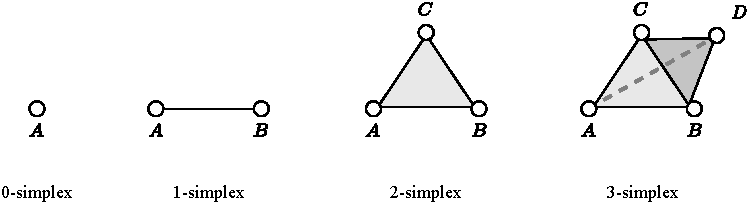
\includegraphics[width=0.9\textwidth]{thesis/figures/n-simplices_cropped.pdf}
    \caption{Building blocks of simplicial complexes, consisting of $n$-simplices.}
    \label{fig:n-simplices-example}
\end{figure}
By combining one or more $n$-simplices, one can create simplicial complexes, as illustrated in \cref{fig:simplicial-complex}.
\begin{figure}[H]
    \centering
    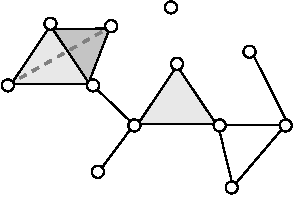
\includegraphics[width=0.5\textwidth]{thesis/figures/simplicial-complex_cropped.pdf}
    \caption{Simplicial complex consisting of $0$-, $1$-, $2$- and $3$-simplices.}
    \label{fig:simplicial-complex}
\end{figure}
There exist several methods for creating simplicial complexes from data. In particular, we will look at the Vietoris–Rips complex in the next sub-subsection.

\subsubsection{Vietoris–Rips complex}
\label{sec:vietoris-rips-complex}
The Vietoris–Rips complex is a simplicial complex that can be created from data points, using any distance metric. Given a proximity diameter $\alpha$, the Vietoris–Rips complex is built by forming a simplex for every set of $k$ data points that have distance less than or equal to $\alpha$. That is, if $k$ data points satisfy $d(x_i, x_j) \leq \alpha$ (where $d(x_i, x_j)$ computes the distance between two data points $i$ and $j$), a $(k-1)$ simplex is created for that data point (1-simplex for two data points, 2-simplex for three data points, etc.). An example of a Vietoris–Rips complex is illustrated in \cref{fig:simplicial-complex-rips}.
\begin{figure}[H]
    \centering
    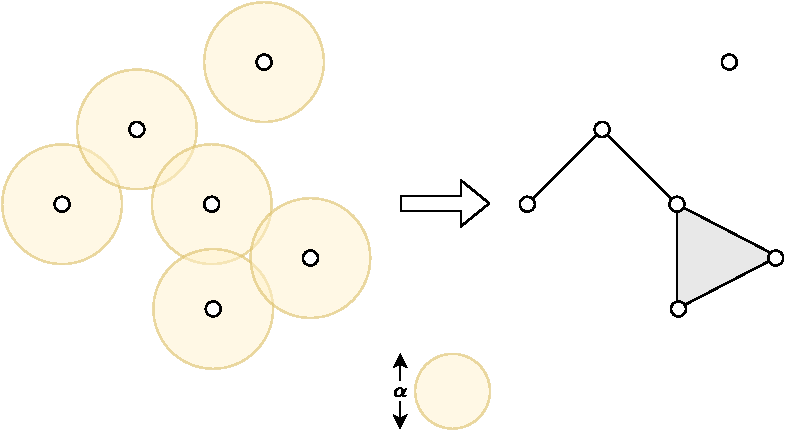
\includegraphics[width=0.7\textwidth]{thesis/figures/simplicial-complex-rips_cropped.pdf}
    \caption{Vietoris–Rips complex on 2-dimensional data with proximity diameter $\alpha$.}
    \label{fig:simplicial-complex-rips}
\end{figure}
By carefully studying the $n$-simplices of a Vietoris–Rips complex, we can observe topological structures such as loops (i.e. $2$-simplices) or holes  (i.e. $3$-simplices). An example of a loop is shown in \cref{fig:simplicial-complex-rips}, where the rightmost data points that the bottom form a 2-simplex. In order to study topological properties of data, it is common to look at varying values of $\alpha$, starting at zero and increasing to infinity. The study of observing how the topology changes once a threshold (e.g. $\alpha$) increases is called persistent homology. In order to easily present and visualize persistent homology, persistence diagrams are used. We will look at persistence diagrams in the next subsection.

\subsection{Persistence diagram}
\label{sec:persistence diagram}
In order to present persistent homology of a simplicial complex, persistence diagrams are frequently used. Persistence diagrams we look at a range of proximity diameters over multiple persistent homology dimensions (or degrees), where the dimension refer to which $n$-simplices we want to look at (0-dimensional persistent homology observe changes of $0$-simplices, 1-dimensional observe changes of $1$-simplices, etc.). A persistence diagram is 2-dimensional, where the x-axis denotes the birth time and y-axis the death time. Assuming that we want to create a persistence diagram of data points, we let the proximity diameter $\alpha$ start at zero. By gradually increasing $\alpha$, new topological properties appear and old topological properties gets merged into other properties. In particular, once a topological property is "birthed" (e.g. 1-simplex between two data points), the birth time is noted for the particular data point. A point in the persistence diagram appear once $n$-simplices gets merged into a new $m$-simplex (e.g. three 1-simplex becoming a 2-simplex).

To motivate the use of persistence diagrams, we show a simple example where we study the change of 0-dimensional persistent homology, illustrated in \cref{fig:persistence-diagram-example}. In \cref{fig:persistence-diagram-example}, we see how the persistence diagram changes once we increase the proximity diameter $\alpha$, on a data set consisting of two blobs. In the first row (a), we let $\alpha=0.2$ and we observe that there are only two data points intersecting, thus leading to a single point in the persistence diagram. In the second row (b), we let $\alpha=1.5$ and we now see that most data points in each blob are connected, thus leading to several entries in the persistence diagram. For the last row (c), we let $\alpha=4.5$, and we observe that there is a single point and several points on the bottom in the persistence diagram. By looking at the plot on the left, we see that the two blobs have now intersected and all data points have connections to other data points with distance less or equal to $\alpha$. In addition to this, the last row (c) indicates that we have two clusters in our data, even though our data was rather noisy and somewhat separated.
\begin{figure}[H]
    \centering
    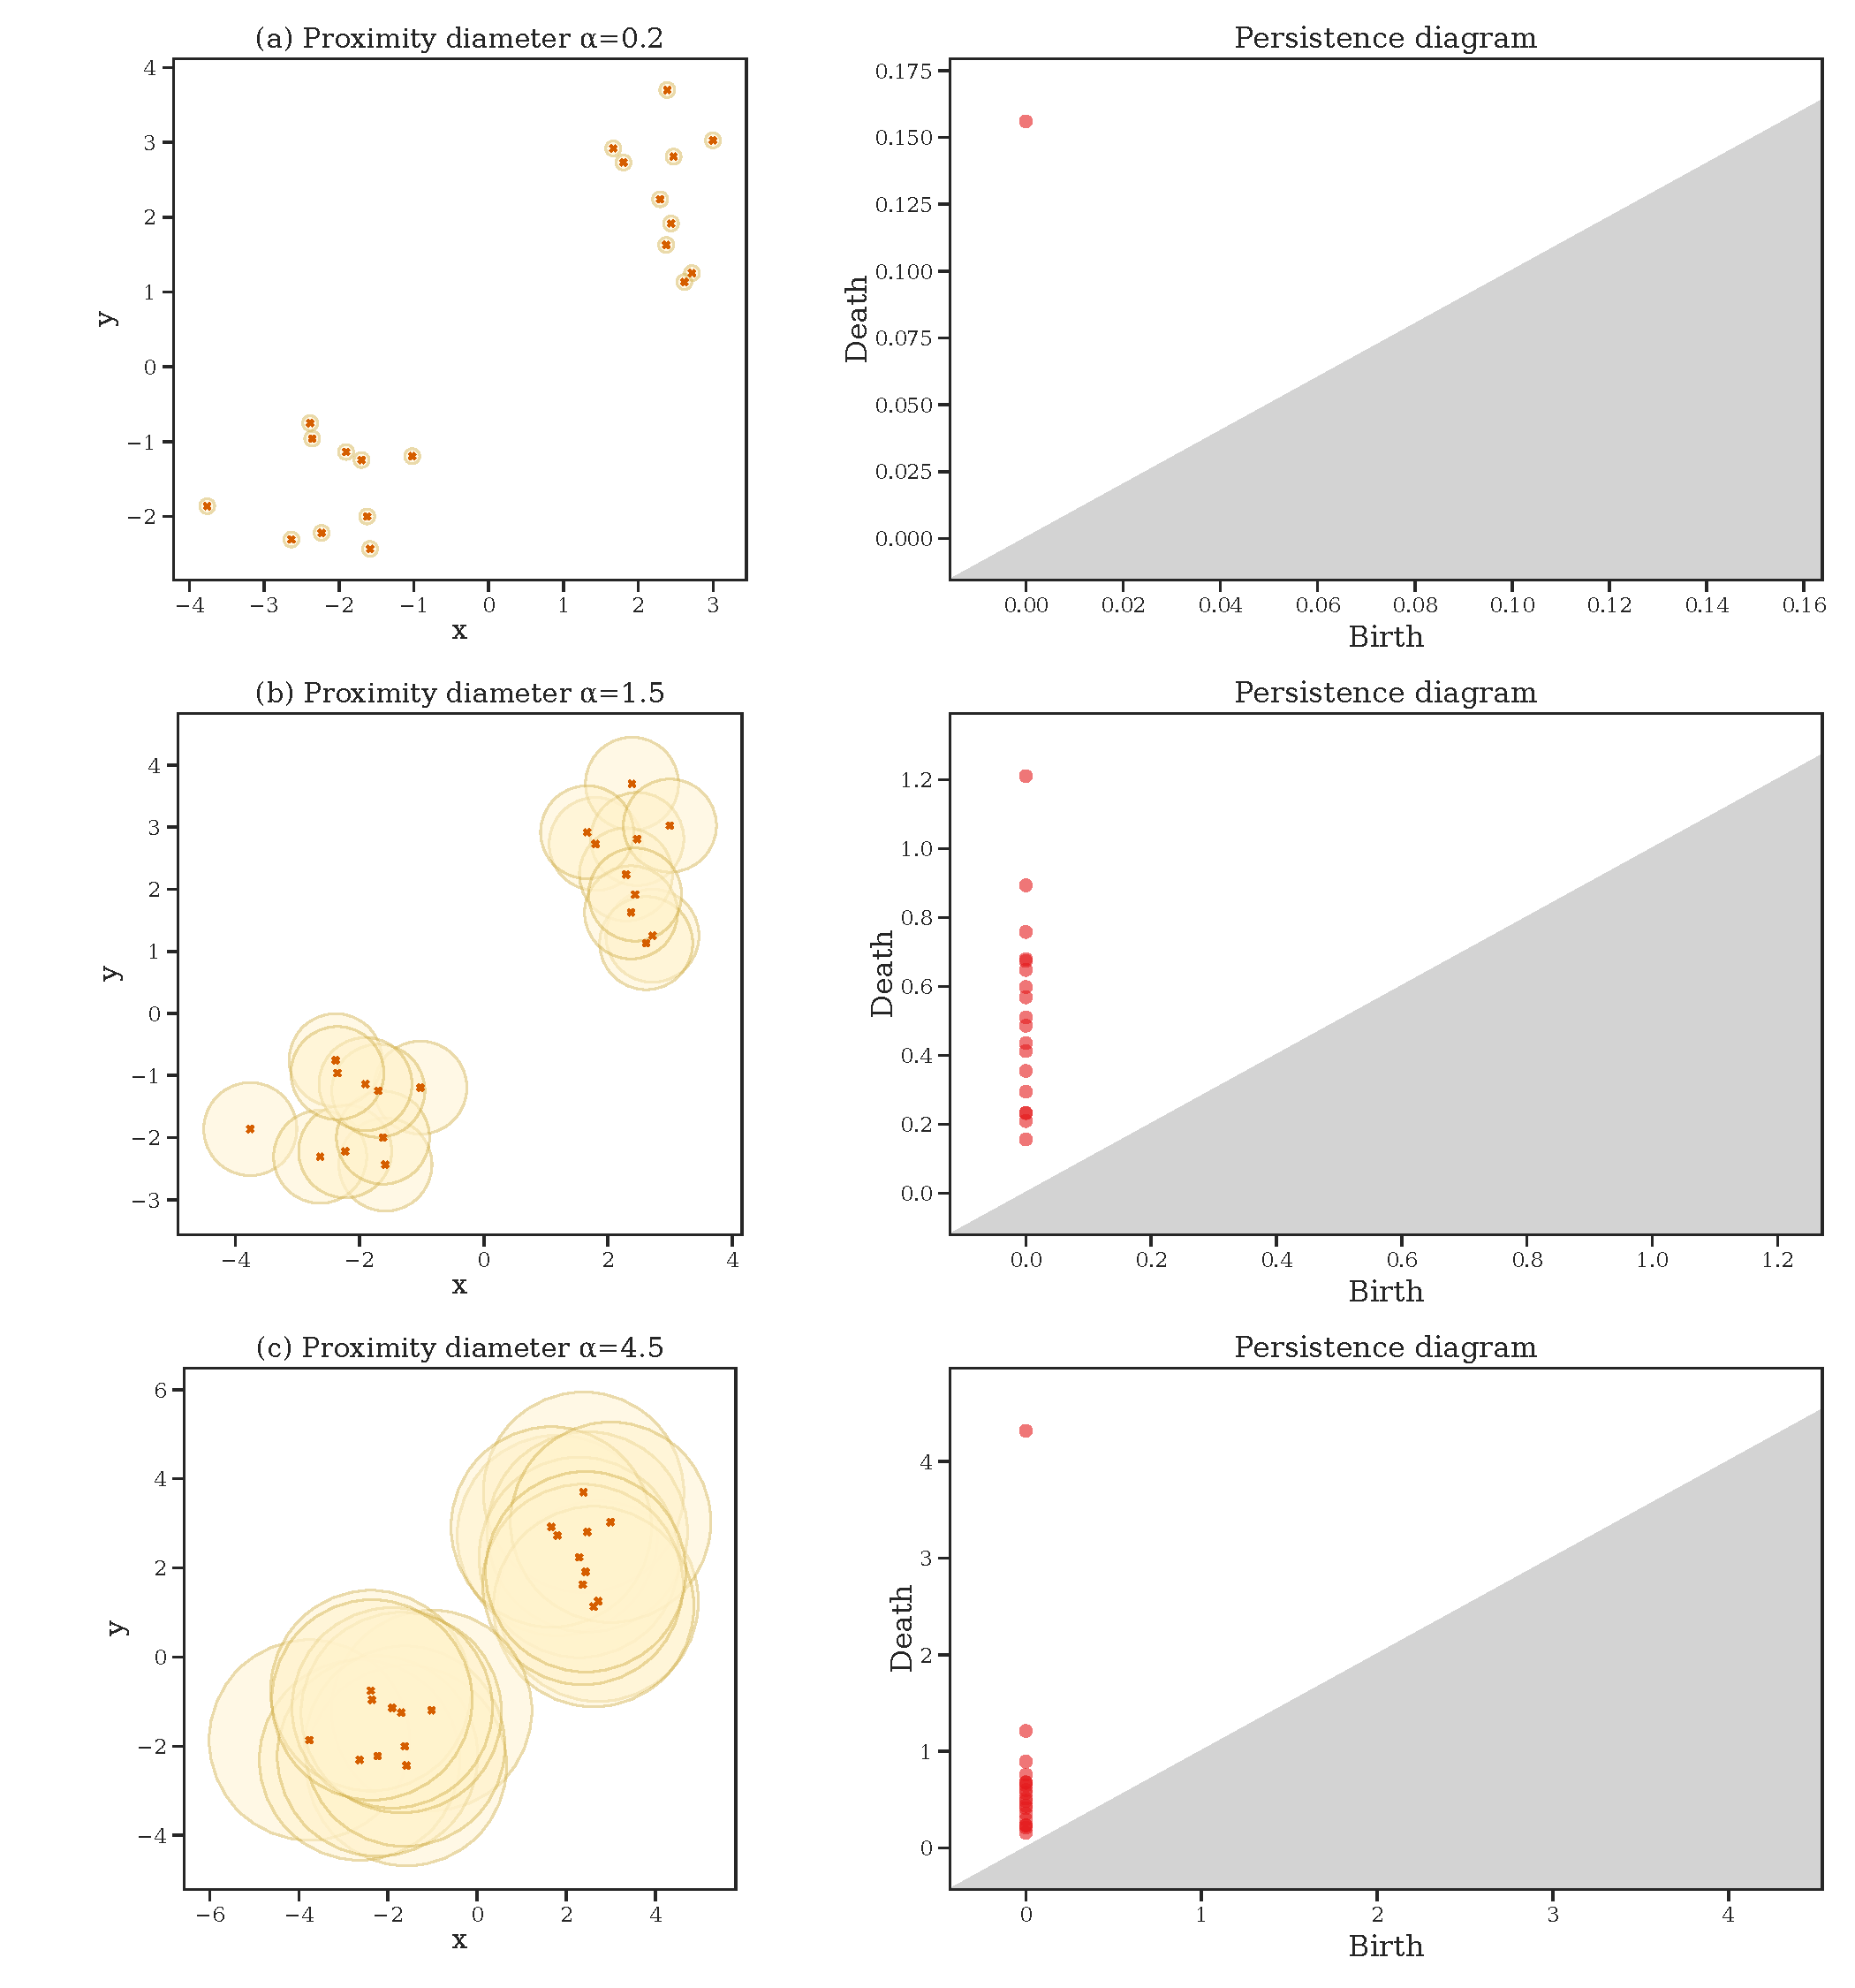
\includegraphics[width=1\textwidth]{thesis/figures/persistence-diagram-example.pdf}
    \caption{Persistence diagrams on different levels of $\alpha$ of a data set consisting of two blobs.}
    \label{fig:persistence-diagram-example}
\end{figure}
An important aspect of machine learning is to predict some quantity given some features. If we want to use the persistence diagrams as features in a model, for instance, a typical approach would be to perform some feature extraction or vectorization first. An example of a vectorization of persistence diagrams are persistence images, which we will introduce in the next subsection.

\subsection{Persistence image}
\label{sec:persistence-image}
Many machine leaning tasks require valuable features in order to yield good results. Persistence images \cite{adams2016persistence} are vector representations of persistence diagrams. When explaining persistence images, we refer to \cite{adams2016persistence}.

Let $B = \enclc{\enclp{b_1, d_1}, \enclp{b_2, d_2}, \ldots, \enclp{b_m, d_m}} \in \R^{m \times 2}$ be a persistence diagram in birth-death coordinates. First, we transform $B$ into birth-persistence coordinates, where persistence is the difference between death and birth. That is, let $T(B) = \enclc{\enclp{b_1, p_1}, \enclp{b_2, p_2}, \ldots, \enclp{b_m, p_m}} \in \R^{m \times 2}$, where $p_i = b_i - d_i$ for $1 \leq i \leq m$. Following, for each of the point in the the $T(B)$ persistence diagram, a probability distribution is placed. A common choice is to use the Gaussian distribution, centered at the respective data point. By placing probability distributions on each point, we are able to differentiate between dense and sparse areas. In addition to placing probability distributions on each point, the distributions are weighted using persistence, making more persistent areas more prominent. Using the weighted probability distributions, for a given persistence diagram $B$ we define the persistence surface of $\rho_B$ as
\begin{align}
    \rho_B(z) = \sumlim{u \in T(B)}{} f(u) \phi_u(z)
\end{align}
where $f(u)$ is the persistence weighing function and $\phi_u(z)$ is the probability distribution evaluated at point $z$ (if Gaussian, then centered at point $u$). Finally, the persistence surface $\rho_B(z)$ is reduced to a discretized representation. In particular, an $N \times M$ grid is formed and for each cell in the grid the integral of $\rho_B(z)$ over that region is computed and used as value. In other words, this discretization allows us to summarize the persistence surface using less information and we are left with an $N \times M$ matrix that can be used for machine learning tasks more easily.

\subsection{Wasserstein distance}
\label{sec:wasserstein-distance}
Distance metrics (e.g. Euclidean distance) are often used to compare distance between data points. In order to compare differences between any two persistence diagrams $A$ and $B$, the $p$\textit{-Wasserstein distance} is often used, as defined in \cref{eqn:wasserstein-distance}.
\begin{align}
    W_p(A, B) = \inf_{\gamma: A \rightarrow B} \enclp{\sumlim{u \in A}{} ||u - \gamma(u)||_{\infty}^{p}}^{1/p}
    \label{eqn:wasserstein-distance}
\end{align}
where $1 \leq p < \infty$ and $\gamma$ ranges over bijections between $A$ and $B$, and $\inf$ is the infimum (greatest lower bound, or similar to "minimum"). If we let $p=\infty$, i.e $W_\infty(A, B)$, we get what we call the \textit{bottleneck distance}. The bottleneck distance is often used to compare persistence diagrams as well, but has the disadvantage of only using the maximum distance between any two points over the bijections between $A$ and $B$.

\subsection{Topological polysemy}
\label{sec:topological-polysemy}
Recall the manifold hypothesis, which states that, in general, real-life high-dimensional data tends to live on a low-dimensional sub-manifold embedded within the high-dimensional space \cite[p. 16]{bengio2014representation}. To give an example, imagine that we have gathered some data about weight and height of humans. Naturally, we see that as the height increases, the weight increases as well. That is, we have a strong linear relationship (or correlation) between height and weight. We can therefore argue that the manifold dimension of the data is 1, even though the original data has dimension 2. The hypothesis should, in theory, also apply to word embeddings, but the authors of \cite{jakubowski2020topology} argue that word embeddings, should instead, live on a punched manifold. By a pinched manifold, we mean a manifold where particular points that are equal in some sense are glued together, creating singular areas in the manifold. An example of a pinched manifold is shown in \cref{fig:pinched-manifold}. For word embeddings, \cite{jakubowski2020topology} claim that these singular areas in the manifold represent polysemous words, where neighbouring words are related to the polysemous word. In order to identify such polysemous words from word embeddings, \cite{jakubowski2020topology} introduce a topological measure of polysemy based on persistent homology, that correlate well with the number of meanings of a word. To explain the topological measure of polysemy, we refer to \cite{jakubowski2020topology}.
\textbf{TODO}: Add figure of pinched manifold.
%\begin{figure}[H]
%    \centering
%    \includegraphics[width=\textwidth]{}
%    \caption{Pinched manifold.}
%    \label{fig:pinched-manifold}
%\end{figure}

Determining the number of word meanings is a non-trivial task. Consider the word \textit{solution}, which has multiple meanings. In some contexts, the word \textit{solution} is related to problems, while in other contexts it could be related to chemistry (mixture of two or more substances). We call such words polysemous, meaning that the word has multiple meanings which are related to one another. The topological measure of polysemy introduced in \cite{jakubowski2020topology} is motivated by the fact that the number of word meanings of a word $w$ should be reflected by the number of components of a punctured neighbourhood around $w$. A punctured neighbourhood of $w$ are neighbouring words of $w$ excluding the word $w$ itself.

Let $W \in \R^{|V| \times d}$ be word embeddings, where $|V|$ is the number of words in the vocabulary and $d$ is the word embedding dimension. Topological polysemy $\text{TPS}_n(w)$ is computed by fixing a target word $w$ and a neighbourhood size $n$. We denote the word vector of $w$ as $v_w \in \R^{d}$. To compute $\text{TPS}_n(w)$, we first normalize the word embeddings $W$ such that each vector are of unit length. The normalized word embeddings are denoted $W_\text{norm}$ and the normalized word vector of the target word $w$ is denoted as $v_{w_{\text{norm}}}$. Following, the punctured neighbourhood $N_n(w)$ is computed, that is, the neighbouring $n$ (normalized) word vectors around $v_{w_{\text{norm}}}$, excluding $w$ itself. Furthermore, we project the word vectors of $N_n(w)$ to lie at the unit sphere, with $v_{w_{\text{norm}}}$ as the center. We denote this normalized punctured neighbourhood as $N'_n(w)$. In other words, we make the word vector of $w$ to be the origin of a $d$-dimensional sphere and project the neighbouring words of $w$ to lie around it. Lastly, the 0-degree persistence diagram of $N'_n(w)$ is computed, denoted $PD_n(w)$. $\text{TPS}_n(w)$ is then the Wasserstein distance between $PD_n(w)$ and the empty persistence diagram, also known as the Wasserstein norm.

\subsection{Geometric Anomaly Detection}
\label{sec:geometric-anomaly-detection}
The manifold hypothesis forms a foundation of modern data science. Many manifold learning and dimensionality reduction algorithms rely on this assumption in order to find meaningful low-dimensional representations of high-dimensional data. Examples of such algorithms include PCA and UMAP. Geometric Anomaly Detection (GAD) \cite{stolz2020geometric} is an algorithm for identifying possible points in data which fail to satisfy the manifold hypothesis. Following, we will describe the GAD algorithm and give a couple of examples of how it works. We refer to \cite{stolz2020geometric} when explaining the GAD algorithm.

To understand how the GAD algorithm works, we will first introduce the motivation behind it. Imagine that we have some data that lies on two submanifolds $P$ and $Q$, as illustrated in \cref{fig:gad-motivation}. Here we assume that the two submanifolds $P$ and $Q$ are planes which intersect at some point, denoted by the dotted red line. We place an annulus around each data point and infer its topological structure. An annulus is the region between two circles, where the first circle is contained in the other and both circles share center point. Annuli can also remind us of rings. Formally, each annulus around its respective data point has an inner radius $r$ and outer radius $s$. Depending on where a point is on either of the submanifolds, we observe that a point can have one of three states as seen in \cref{fig:gad-motivation}: (a), (b) or (c). If a point is at the boundary of either submanifolds, i.e. situation (a), we observe that the points falling into the annulus around the data point forms a half circle, as half of the circle does not have any data points in them. If we count the number of topological loops we get zero. If the data point falls nicely into either submanifold, i.e. situation (b), we observe that we get a nice annulus where neighbouring points falling into the annulus around the data point forms a circle. In other words, if a point is on the submanifold, we expect to get exactly one topological loop. For the last situation, i.e. (c), we have a data point which falls between $P$ and $Q$, creating a singularity (or anomaly) in the data. This stamps from the fact that it harder to distinguish which submanifold the particular data point should belong to. If we look at the data points in the annulus around the data point, we observe that we get two or more topological loops.
\begin{figure}[H]
    \centering
    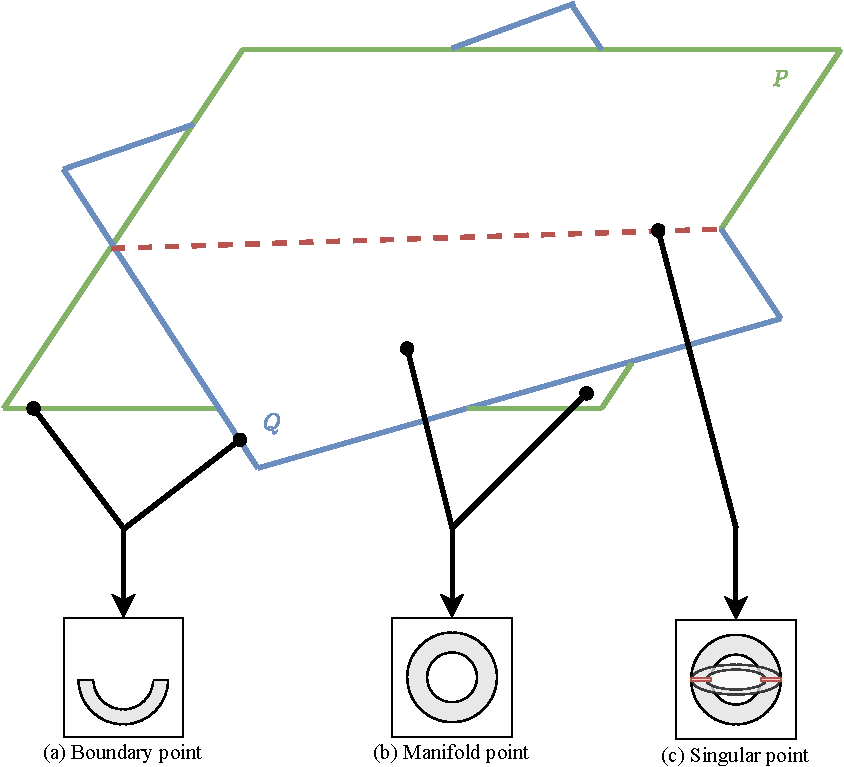
\includegraphics[width=0.8\textwidth]{thesis/figures/geometric-anomaly-detection-motivation_cropped.pdf}
    \caption{Motivation behind the GAD algorithm. Data points belonging to two submanifolds $P$ and $Q$, and depending on where the data points are on the submanifolds, it can have three different states: (a), (b) or (c). The GAD algorithm is particularity interested in finding singular (c) data points between $k$ submanifolds (here: $k=2$). This illustration is inspired by \cite[Figure 1]{stolz2020geometric}.}
    \label{fig:gad-motivation}
\end{figure}

Let $X \in R^{n \times d}$ be data points. The GAD algorithm works as follows: fix two parameters $0 < r < s$, and for each data point $x_i \in X$ place an annulus around it, with inner radius $r$ and outer radius $s$. Determine the data points that fall into the annular neighbourhood of $x_i$ and denote this set as $A_y = \enclc{a_1, a_2, \ldots, a_m} \subset X$. That is, the set $A_y$ consists of those points $a_j$ that satisfies $r \leq d(x_i, g_j) \leq s$, where $d(\cdot, \cdot)$ measures the distance between two points (e.g. using Euclidean distance). Then, select a manifold dimension $k$ we would like to investigate, as the GAD algorithm discovers intersections of $(k-1)$ submanifolds. In order to find intersections of $(k-1)$ submanifolds of the annular neighbourhood $A_y$ of $x_i$, we compute the $(k-1)$-dimensional Vietoris–Rips complex of $A_y$, denoted $VR_{k-1}(A_y)$. Then, for each birth-death coordinate $(b_{k-1}, d_{k-1}) \in VR_{k-1}(A_y)$, we count the number of points that persist longer as the annulus width, denoted $N_y$. Recall that the persistence of points in persistence diagrams can be computed by transforming the persistence diagram into birth-persistence coordinates, where persistence $p_{k-1} = d_{k-1} - b_{k-1}$. We define the annulus width to be the difference between the outer and inner radius, i.e. $w_{A_y} = s - r$. To count $N_y$, we iterate over the points in the persistence diagram and count the number of points that satisfies
\begin{align}
    p_{k-1} > w_{A_y}
    \label{eqn:gad-ny-condition}
\end{align}
The count $N_y$ is analogous to the number of topological loops that occur in $A_y$ for a given homology dimension $(k-1)$. If no points satisfy \cref{eqn:gad-ny-condition}, i.e. $N_y=0$, then $x_i$ is classified as a boundary point, similar to the (a) situation in \cref{fig:gad-motivation}. If we have exactly one point that satisfies \cref{eqn:gad-ny-condition}, i.e $N_y=1$, then the point is classified as a boundary point, similar to the (b) situation in \cref{fig:gad-motivation}. If two or more points satisfy \cref{eqn:gad-ny-condition}, i.e. $N_y>1$, then the point is classified as a singular point, similar to the (c) situation in \cref{fig:gad-motivation}.